\section{2D pose estimation}
The foremost step in Human Pose Estimation (HPE) is to model the human body entity representing its kinematic structure and shape information. In recent studies, benefiting from the intuitive nature of graph representations, the human body structure has been characterized by anatomical joints and their positions \cite{zuffi_pictorial_2012}. This approach is known as the kinematic model (Shown in \autoref{fig:pose-modeling} a), and is widely employed to describe human poses. In 2D Human Pose Estimation, the goal is to localize the 2D position or spatial location of human body keypoints (kinematic joints) from the input data \cite{rafi_efficient_2016}.

\begin{figure*}[!htb]
	\centering
	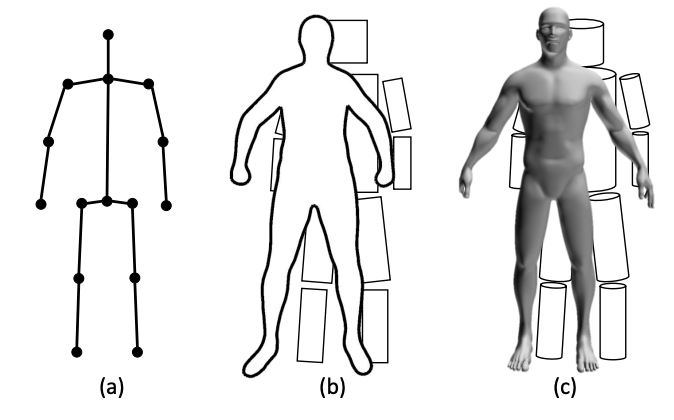
\includegraphics[scale=0.6]{2dpose/human-modeling}
	\caption{Human body modeling. (a)kinematic-based model; (b)contour-based models; (c)volume-based models. 
	\cite{chen_monocular_2020}}
	\label{fig:pose-modeling}
\end{figure*}

Recently, deep neural networks have achieved a significant breakthrough in 2D HPE and are mainly employed to extract robust features for keypoint recognition and localization directly from the input data (images and videos). Since the quality of feature representation is intimately tied to network architecture, the subject of network design was chosen to be thoroughly investigated. 

\subsection*{HPE Network Architecture Design Challenges}

Like many tasks in computer vision (e.g., object detection, image segmentation, etc.), the primary technological challenges in developing 2D HPE algorithms are the accuracy and efficiency of the proposed method. High precision pose estimation facilitates accurate human body information for subsequent tasks, including lifting from 2D to 3D HPE models. In addition to the accuracy of an HPE algorithm, its efficiency (inference speed) is also desired for real-time applications. However, there is mostly a trade-off between accuracy and efficiency concerning algorithm development since the high accuracy methods tend to be more complex and demand powerful resources for computation. Consequently, lightweight models with comparable precision are more desirable for mobile or wearable devices. 

Another crucial challenge in 2D HPE is estimating poses for multi-person scenarios. 2D single-person HPE localizes joint coordinates when only one human instance is in the input image, but for images containing multiple persons, the HPE model needs to recognize each human in the input image before estimating its keypoints positions. This process can be done by a two-stage process called the top-down approach that first detects individual persons, i.e., the input image is divided into sub-images (patches) enclosing just one person \cite{sun_deep_2019}. Then the deep learning keypoint detection algorithm can be applied to each patch. On the other hand, there is an alternative group of approaches known as bottom-up, in which human joints are detected directly from the image without an explicit object detection stage \cite{cheng_higherhrnet_2020}. The following sections will review current frameworks utilizing top-down and bottom-up approaches to their network architectures.

\subsection{Top-Down Framework}

The top-down approaches employ human body detectors \cite{ren_faster_2016, micilotta_real-time_2006} to obtain a set of bounding boxes (each corresponding to one person) from the input images and then perform pose estimation within each bounding box. The existing literature in 2D HPE based on top-down approaches can also be divided into fine-grained sub-categories discussed in this section: regression-based and heat map-based approaches. 

\subsubsection{Regression-based methods}

There are many works based on the regression technique \cite{carreira_human_2016, fan_combining_2015, fieraru_learning_2018, li_heterogeneous_2014, qiu_peeking_2020, sun_compositional_2017, sun_integral_2018, toshev_deeppose_2014, wang_graph-pcnn_2020,z} that directly regress human body joint coordinates via an end-to-end trained network that maps the input image to the pre-defined graphical structures (kinematic keypoints). Accordingly, the regression hypothesis is defined as follows:

Given an image I, the goal of pose estimation is to predict a possibly empty set of human instances, $\{Pi\}_{i=1}^N$ where \textbf{\textit{N}} is the number of persons in the image. For each person, we need to predict its bounding box information, $\{Bi\}$, as well as its keypoint coordinates, $Ki=\{(x_j, y_j)\}_{j=1}^J$, where \textbf{\textit{J}} is the number of pre-defined joints in each dataset \cite{li_pose_2021}.

DeepPose \cite{toshev_deeppose_2014} is a regressor that explicitly predicts human joint locations through fully connected layers of a deep neural network. AlexNet \cite{krizhevsky_imagenet_2012} as the backbone of DeepPose's cascaded architecture for feature extraction. Due to the remarkable performance of DeepPose in efficient keypoint detection by using convolutional neural networks (CNNs), human pose estimation techniques have gradually migrated from the conventional graphical models to deep learning approaches. 

Carreira et al. \cite{carreira_human_2016} proposed a model based on GoogLeNet \cite{szegedy_going_2014} that adopts an iterative feedback mechanism called Iterative Error Feedback (IEF) to enhance the efficiency of hierarchical feature extractors such as Convolutional Networks (ConvNets) in early layers. This self-correcting model progressively adjusts an initial estimate of joint coordinates by feeding back predictions error in the IEF process instead of directly predicting the coordinates in a feed-forward network.

Transformer models \cite{vaswani_attention_2017} based on the self-attention mechanism have significantly advanced the field of representation learning and promoted visual understanding tasks such as object detection frameworks that are free of region proposals, anchors, and post-processing (non-maximum suppression) procedures. In a recent study \cite{li_pose_2021}, authors took full advantage of the tokenized representation in transformers with self-attention layers. They propose a regression-based human pose estimation method, called pose recognition Transformer (PRTR), using two types of cascade transformers based on an end-to-end object detection Transformer (DETR) \cite{carion_end--end_2020}. In this proposed model, the second transformer is a regressor that predicts joints' coordinates within each image patch detected from the first transformer and performs multi-person pose estimation. PRTR reveals competitive results for pose recognition compared with other existing regression-based methods on the challenging COCO dataset.


\subsubsection{Heatmap-based Methods}

In the field of human pose estimation, heatmap-based approaches seek to train a deep neural network to approximate the locations of body parts and joints based on heatmap representations \cite{chen_articulated_2014, newell_stacked_2016, wei_convolutional_2016}. Accordingly, during training, the pose estimation model generates J heatmaps $\{Hj\}_{j=1}^J$, as a 2-dimensional Gaussian distribution centered at the ground-truth joint location, where J is the total number of joints. The pixel value $Hj \{(x_i,y_i)\}$ in each joint heatmap encodes the probability that the $j^{th}$ joint lies in the location $(x,y)$  \cite{tompson_efficient_2015, tompson_joint_2014}. 

The probability values provide richer supervision that facilitates the training of convolutional networks and significantly improves the performance of heatmap-based over regression-based approaches \cite{artacho_unipose_2020, bulat_human_2016,gkioxari_chained_2016, lifshitz_human_2016,newell_stacked_2016,tompson_efficient_2015}. Therefore, heatmaps preserve the spatial location information of joints and reduce the number of false-positive cases, which results in an increasing attraction to develop deep learning pipelines for HPE based on heatmap representations \cite{carreira_human_2016,luo_lstm_2018,toshev_deeppose_2014,wei_convolutional_2016}.

Ramakrishna et. al \cite{ramakrishna_pose_2014} presented a sequential prediction framework based on convolutional networks named Convolutional Pose Machines (CPM) that learns rich implicit spatial structures by utilizing the inference machine framework to incrementally refine estimates of the human body part (e.g., head, leg, etc.) locations in multiple stages. In this method, a predictor is trained to predict the confidence of the body part locations in each stage. In the first stage, the predictors estimate the confidence of each part location from heatmaps computed on the input image patch. Since a heatmap produced only from image features is noisy and has multiple modes, in the subsequent stage, the network iteratively refines the estimated confidences using contextual information from outputs of the previous stage. 

In a further expanding of Pose Machine architecture, \cite{wei_convolutional_2016} employed sequential convolutions to implicitly model long-range spatial relationships between different parts. It is worth mentioning that multiple stages increase the network depth and make it hard to train because of the vanishing gradient problem ---as the gradient is back-propagated to the layers of earlier stages, repeated multiplication makes the gradient infinitely small. Thus, as the network goes deeper, its performance gets saturated or degrades rapidly. 

Before ResNet \cite{he_deep_2016}, there were several methods to deal with the vanishing gradient issue; for instance, the authors of this work \cite{wei_convolutional_2016} developed an auxiliary loss in a middle layer as extra supervision. But this can not tackle the problem entirely since each stage will fail to extract robust semantic features from the input data and is prone to overfitting. The core idea of ResNet is introducing "shortcut connections" that skip (jump over) one or more layers. These skip connections effectively simplify the network and reduce the impact of vanishing gradients as it allows the back-propagation of training errors at deeper levels (addressing the issue of iterative architectures with multiple stages). Residual networks dramatically improved the 2D HPE process, and numerous models
\cite{cai_learning_2020, chen_cascaded_2018, chu_multi-context_2017, ke_multi-scale_2018, liu_cascaded_2018, newell_stacked_2016, su_multi-person_2019, sun_deep_2019, xiao_simple_2018-1, yang_learning_2017} have been developed due to their advantage. 

An encoder-decoder network called "stacked hourglass" (SHG) based on the sequential stages of pooling and upsampling layers was presented by Newell et al. \cite{newell_stacked_2016} to capture spatial correlations between the human body keypoints by combining low and high-resolution feature representations. Several more complicated variants have been introduced following the initial success of SHG architecture; specifically, Chu et al. \cite{chu_multi-context_2017} developed novel Hourglass Residual Units (HRUs) extended by a side branch of filters with larger receptive fields that learn features across various scales. Yang et al. \cite{yang_learning_2017} replaced the residual units in SHG with multi-branch Pyramid Residual Modules (PRMs) to enhance deep convolutional neural networks by constructing scale invariance features. 

Cai et al. \cite{cai_learning_2020} recently proposed the Residual Steps Network (RSN), which efficiently maintains rich low-level spatial information by aggregating intra-level features with the same spatial size to localize the keypoints precisely using delicate local representations. In addition, they devised a novel attention mechanism, Pose Refine Machine (PRM), that refines the keypoint locations by finding a trade-off between the contribution of local and global representations in the resultant feature. Their approach accomplished state-of-the-art results on COCO and MPII benchmarks and won 1st place in the COCO Keypoint Challenge 2019.


\subsection*{Top-Down Approaches Summary}

The primary components of top-down frameworks in human pose estimation consist of an object detector and a pose estimator to predict the joint positions of the human body. The object detector determines human proposal detection performance and influences pose estimation. On the other hand, the pose estimator component is the framework's heart that directly affects the pose estimation accuracy. The main reason for adopting heat map-based and regression-based methods for the pose estimator component is the speed-accuracy trade-off. 

In regression-based human pose estimation, the problem is formulated as a regression one in which features extracted from convolution layers of a CNN are regressed to directly predict joint coordinates of the body parts. The regression-based networks can be trainable end-to-end and are efficient in real-time applications since they have fewer intermediate non-differentiable steps \cite{liu_cascaded_2018, eichner_human_2012, felzenszwalb_pictorial_2005, girdhar_detect-and-track_2018}; however, they typically perform less accurately than heat map-based approaches. Because when the body parts are not completely visible, they fail to accurately estimate the locations of human body joints. To address this shortcoming, probabilistic heatmaps are employed to learn a complex mapping from occluded part appearances to joint coordinates instead of directly regressing them. 

Human pose estimation based on heatmaps comprises pre-processing and post-processing procedures to encode keypoints' ground truth (GT) into heatmaps and decode heatmaps to predict joint locations. Consequently, they can be optimized easier and in comparison to regression-based methods, have a more robust generalization that delivers substantial performance, primarily suitable to be adopted when accuracy is the priority \cite{pfister_flowing_2015}. Nevertheless, heatmap-based frameworks have various heuristic network designs that are mostly not end-to-end learnable and suffer from several shortcomings: Firstly, to generate the 2D heatmaps, computationally expensive upsampling operations (e.g., deconvolution layers in \cite{yixing_gao_user_2015}) are required. Also, an extra post-processing step for reducing projection errors from heatmap to ground truth coordinates is unavoidable in further keypoint estimation refinements. This makes them sub-optimal, i.e., the speed efficiency (performance) of heatmap-based methods usually declines drastically as the input image resolution decreases. 

\subsection{Bottom-Up Framework}
 
After analyzing the top-down frameworks in the network architecture design context for human pose estimation, it is noteworthy to consider the bottom-up approaches. These approaches (e.g.,\cite{micilotta_real-time_2006, cheng_higherhrnet_2020, fieraru_learning_2018, jin_differentiable_2020, kreiss_pifpaf_2019, nie_single-stage_2019,insafutdinov_arttrack_2017, insafutdinov_deepercut_2016, newell_associative_2017, pishchulin_deepcut_2016, tian_directpose_2019} aim to perform two main tasks: firstly, human keypoint detection through extracting local features from the input image and proposing a set of human body joint candidates, and then grouping those candidates to build pose representations for each individual person. 

The main distinguishing characteristic of the bottom-up approach from the former approach is that the framework design does not rely on a human detection component to predict human bounding boxes separately. As a result, the computational overhead decreases substantially by directly estimating human poses from extracted features; however, the major challenge is an identification mechanism for estimated keypoints to associate different subsets of candidates to each individual human body. Accordingly, we can divide research studies on the Bottom-Up HPE into three subgroups as human center regression \cite{geng_bottom-up_2021, nie_single-stage_2019, nie_human_2018}, part field \cite{jin_differentiable_2020, kreiss_pifpaf_2019, martinez_single-network_2019, insafutdinov_deepercut_2016, li_simple_2019}, and associate embedding \cite{cheng_higherhrnet_2020, jin_multi-person_2019, luo_rethinking_2021, newell_associative_2017} approaches. 

\subsubsection{Human Center Regression}

In the human center regression-based approach, a center point is defined as representative of humans. In a study, the authors developed a novel model called Pose Partition Network (PPN) \cite{ferrari_pose_2018} with the stacked hourglass architecture \cite{newell_stacked_2016} as the backbone that simultaneously detects keypoints and performs dense regressions from global joint candidates to robustly generate joint partitions within a specific embedding space parameterized by centroids of persons. PPN improved multi-person pose estimation using a local greedy inference approach, resulting in low computation cost and accurate joint detection.

One year later, Nie et al. presented the advantage of a Single-stage Pose Machine (SPM) \cite{nie_single-stage_2019} using the Hourglass network architecture in enhancing the efficiency of multi-person pose estimation over the conventional two-stage approaches. To achieve this, they proposed a novel  Structured Pose Representation (SPR) model in which the root (centered) keypoints indicate each human body instance, and then other body joint locations are encoded into their displacements w.r.t. the roots. Accordingly, SPM demonstrated state-of-the-art efficiency and outstanding accuracy for multi-person 2D and 3D human pose estimation compared to other methods on multiple benchmark datasets such as COCO.

Recently, Geng et al. \cite{geng_bottom-up_2021} studied the keypoint regions for regressing keypoint positions accurately. They employed a multi-branch network that indicates the human body instances by predicting a human center map and densely estimates a candidate pose at each pixel q within the consequent map. This direct regression approach is called Disentangled Keypoint Regression (DEKR) and shows higher accuracy than the superior bottom-up pose estimation methods on the COCO dataset.

\subsubsection{Part Field}
 
The part-field method is another subgroup of the bottom-up approaches pioneered by a model named OpenPose \cite{cao_realtime_2017}, which first detects keypoints and connections between them and then performs keypoint grouping according to the connective intensity between different keypoints. This approach uses Convolutional Pose Machines \cite{wei_convolutional_2016} and proposes a two-branch multi-stage architecture, where the detector branch predicts keypoints’ coordinates via heatmaps. In parallel, the other represents the Part Affinity Fields (a set of 2D vector fields with vector maps) to denote the position and orientation of human body parts and associate them with each person. As a result, OpenPose achieved a real-time performance among bottom-up multi-person human pose estimation methods regardless of the number of persons in the image; however, it showed an inferior performance with low-resolution images and occlusions. 

To address this problem, many studies were proposed to improve the OpenPose structure. For example, Zhu et al. \cite{zhu_multi-person_nodate} adopted redundant edges to increase the intensity of connections between joints in PAFs and obtained better performance than the baseline approach. Kreiss et al. \cite{kreiss_pifpaf_2019} proposed a method called PifPaf that employed a Part Intensity Field (PIF) to localize body parts, along with Part Association Field (PAF) to associate body parts with each other. This method outperformed previous OpenPose-based approaches based on a box-free, single-shot, fully convolutional network architecture. 

\subsubsection{Associate Embedding} 

Motivated by OpenPose \cite{cao_realtime_2017} and stacked hourglass structure \cite{newell_stacked_2016}, the associate embedding approach in bottom-up human pose estimation was initially introduced by Newell et al. \cite{newell_associative_2017}, where an embedding vector is assigned to each detected keypoints and acts as an identifier tag for associating keypoints to its human body instance. They trained a single-stage deep convolutional neural network that performs keypoint detection and grouping simultaneously. Their results exhibited a remarkable performance on the COCO dataset. Inspired by the keypoint grouping procedure in OpenPose, Cheng et al. \cite{cheng_higherhrnet_2020} devoted to improving the bottom-up pose estimation for small human body instances in the input image by suggesting an extension of HRNet, to yield high-resolution features pyramids. Their approach, Higher Resolution Network, deconvolves the high-resolution heatmaps generated by HRNet and tackles the scale variation problem in bottom-up multi-person HPE. 

Jin et al. \cite{jin_multi-person_2019} proposed a multi-person pose estimation and tracking pipeline that encloses two sub-networks, SpatialNet and TemporalNet. In this approach, body part detection, keypoint embedding prediction, and part-level data association are driven by the SpatialNet, while the TemporalNet is responsible for pose tracking. One year later, the authors proposed a novel method, called Differentiable Hierarchical Graph Grouping \cite{jin_differentiable_2020}, to learn the human part grouping based on alternative representations of keypoint connection for keypoint grouping. They argued that the separate keypoint grouping mechanism in bottom-up approaches is not end-end trainable, making their performance sub-optimal. To solve this issue, they modeled the human body pose using graph-structured data (nodes and edges) to represent keypoints and their relationships and deliver a fast and scalable (computationally efficient) end-to-end trainable network for detecting and grouping human body joints. 

According to a recent study \cite{luo_rethinking_2021}, bottom-up methods based on heatmap regression suffer from significant variance in human scales and labeling ambiguities of ground truth heatmaps because they are usually generated by 2D Gaussian kernels that have fixed standard deviations. To tackle these issues, the authors proposed the scale-adaptive heatmap regression (SAHR) method along with the weight-adaptive heatmap regression (WAHR) to deliver a model that is more resilient to various human scales and labeling ambiguities via adaptively adjusting the standard deviation for each keypoint. As a result, this framework improved the accuracy of human pose estimation by +1.5AP and outperformed the state-of-the-art top-down methods on the COCO dataset with 72.0 AP.


\subsection*{Bottom-up Approaches Summary}

Top-down approaches deliver high performance in human pose estimation; however, the number of individuals in the input image directly affects their computation efficiency. Bottom-up methods are usually faster than top-down methods since they first locate all keypoints and then group them to their corresponding person; thus, they are computationally more efficient without requiring to estimate the pose for each person separately. 

 
\subsection{2D Human Pose Estimation Summary}


In summary, with the advent of deep neural networks, methods such as DeepPose \cite{toshev_deeppose_2014}, Stacked Hourglass Network \cite{newell_stacked_2016}, and OpenPose \cite{cao_realtime_2017} enhanced the performance of 2D HPE significantly; however, several challenges like human body detection in crowd scenarios \cite{chen_cascaded_2018} still need to be further addressed in future research. In top-down 2D HPE methods, human body detection modules may fail to recognize different persons due to the non-max suppression mechanism that suppresses a valid instance when multiple human bodies are spatially close in the input image, and their boundaries are highly overlapped. Likewise, the keypoint grouping procedure in bottom-up approaches is prone to fail in occluded scenes. Another challenge is computing speed. Although some methods like OpenPose \cite{cao_realtime_2017} can achieve near real-time processing on GPU processors (22 FPS), they are not still efficient for resource-constrained devices, e.g., mobile phones.